%\documentclass[a4paper,twocolumn]{article} % Document type

\documentclass[a4paper,12pt,oneside,onecolumn]{article} % Document type

\usepackage[left=1.0in, right=1.0in, top=1.0in, bottom=1.0in]{geometry}

\ifx\pdfoutput\undefined
    %Use old Latex if PDFLatex does not work
   \usepackage[dvips]{graphicx}% To get graphics working
   \DeclareGraphicsExtensions{.eps} % Encapsulated PostScript
 \else
    %Use PDFLatex
   \usepackage[pdftex]{graphicx}% To get graphics working
   \DeclareGraphicsExtensions{.pdf,.jpg,.png,.mps,.eps} % Portable Document Format, Joint Photographic Experts Group, Portable Network Graphics, MetaPost
   \pdfcompresslevel=9
\fi
\usepackage{gensymb}
\usepackage{amsmath,amssymb}   % Contains mathematical symbols
\usepackage[ansinew]{inputenc} % Input encoding, identical to Windows 1252
\usepackage[english]{babel}    % Language
\usepackage[square,numbers]{natbib}     %Nice numbered citations
\bibliographystyle{plainnat}            %Sorted bibliography



\begin{document}               % Begins the document

\title{Homework 3 in EL2450 Hybrid and Embedded Control Systems}

%\date{2010-10-10}             % If you want to set the date yourself.

\maketitle                     % Generates the title




%%%%%%%%%%%%%%%%%%%%%%%%%%%%%%%%%%%%%%%%%%%%%%%%%%%%%%%%%%%%%%%%%%%%%%%%%%%%%%%%%%%
% Instructions regarding the report
%%%%%%%%%%%%%%%%%%%%%%%%%%%%%%%%%%%%%%%%%%%%%%%%%%%%%%%%%%%%%%%%%%%%%%%%%%%%%%%%%%%

%\section*{Instructions and Help}
%
%\textbf{Please remove this part and the sample references before submitting your homework.}
%
%Read the general homework instructions available on the course homepage before starting to write the report.
%
%Here are some additional guidelines how to write a homework report.
%\begin{itemize}
% \item Fill in name and personal number of all group members.
% \item Do not copy the task descriptions and use the structure below.
% \item Do not include code unless the task explicitly states so.
% \item Motivate your answers well and how you derived them, but be concise.
% \item The number of points is not necessarily related to much you need to write for task.
% \item Put references in the end if any.
% \item Do not include plots from the Simulink scope (color on black background) but export the data to Matlab for plotting.
% \item Include graphics directly in the text and not in a Figure environment, as you normally would. That makes it easier to correct the report.
% \item There is plenty of material available how to use Latex. Use a search engine of your choice to learn more.
%\end{itemize}
%
%Here are some examples how to use Latex:
%\begin{itemize}
% \item An equation with a reference \eqref{eq_sample} to it
% \begin{equation}
%  \dot{x} = \frac{3}{4} x. \label{eq_sample}
% \end{equation}
% \item A multi-line equations with a reference to it
% \begin{align*}
%  \hat{x} &= x - y\\
%  \alpha &= x + \gamma.
% \end{align*}
% \item An equation in text: $\Phi = \int\limits_{0}^{h} \mathrm{e}^{A\tau} d \tau$.
% \item An image
% \begin{center}
%  \includegraphics[width = 0.8\textwidth]{Phase_portrait_with_regionmark}
% \end{center}
% \item A table
% 
% \begin{tabular}{@{\vrule height 10.5pt depth4pt  width0pt}|c|c|c|c|}
%    \hline
%     $-2.46$ & $0$ & $-1.73$ & $0$ \\ \hline
%     $0$ & $-2.553$ & $0$ & $2.774$ \\ \hline
%     $0$ & $6.172$ & $-10$ & $7.333$ \\ \hline
%     $1.767$ & $-0.357$ & $5.714$ & $-6.074$ \\ \hline
%  \end{tabular}
%  \item A citation \cite{Oetiker:2008:TheNotSoShortIntroductiontoLaTeXe}
%  \item Display something exactly as it is written: \verb|\frac{1}{2}_|
%  \item Basic formating: \textbf{bold}, \textit{italics}, \texttt{typewriter}
%\end{itemize}
%
%
%
\section*{Task 1}
The robot is modelled as follows
\begin{subequations}
\begin{equation}
\label{eq:xdot}
\dot{x} = R u_\omega cos\theta
\end{equation}
\begin{equation}
\label{eq:ydot}
\dot{y} = R u_\omega sin\theta
\end{equation}
\begin{equation}
\label{eq:thetadot}
\dot{\theta} = \frac{R}{L} u_\psi
\end{equation}
\end{subequations}

We can write them as
\begin{equation}
u_r = u_{\omega} + \frac{u_{\psi}}{2}
\end{equation}
and
\begin{equation}
u_l = u_{\omega} - \frac{u_{\psi}}{2}
\end{equation}

\section*{Task 2}

The true values of \texttt{R} and \texttt{L} are $R_{true} =0.10014 $ and $L_{true} = 0.505286$. We're solving $R$ from the differential equation for $\dot{x}$ as
\begin{equation}
\label{eq:R}
R = \frac{\dot{x}}{u_{\omega}cos(\theta)}
\end{equation}
where $u_{\omega} = 200$. We get the derivative of $x$ by fitting a line to the data for $x$ in \texttt{forward.csv}, then get $R$ by taking the mean of equation \ref{eq:R}. The result is $R = 0.00100574$, which obviously is off by two orders of magnitude. From there we apply the same solution to $\dot{\theta}$ to get $L = 0.50769$ although we used our $R$ multiplied with the factor $100$.

\section*{Task 3}

The control system in this question can be assumed to be a bang bang or on-off controller operating in a relay manner.  Zeno behaviour is known as an infinite number of steps of a variable within a finite amount of time and can often be difficult to control within a hybrid system.\\
\\
When simulating a system with such a behaviour in Matlab it will cause a lot of "chatter" or oscillation around the operating point, which leads to the solver being unable to solve the system. This is observed in this simulation at around 1 second and therefore the system cannot be observed to be stable within the simulation.\\
\\
Judging by the later questions, i.e. question 4, it is likely that the system has an extremely small error oscillation around zero and is not asymptotically stable in theory.\\
\\
In practice this will be an extremely small value.

 \begin{center}
  \includegraphics[width = 0.8\textwidth]{q3plot}
 \end{center}

 
\section*{Task 4}

The control system in this question can be assumed
to be a bang bang or on-off controller operating in a relay manner with a time delay. The system appears to converge to zero, the time delay added in this section now means that the system can be simulated unlike the first rotation simulation.\\
\\

The downside to this is that Zeno-like behaviour again develops, with continuous switching between control
input of -1 and 1. Asymptotic stability cannot be shown under close observation as the output fluctuates between extremely small positive and negative numbers. This is not a montonically decreasing function so it cannot have finite value as time goes to infinity.\\
\\

This is not an infinite number of steps, condition for Zeno behaviour, though clearly as the solver can now solve the simulation. This is, however, extremely hard on the actuators and is behaviour that should be avoided.\\
\\

 \begin{center}
  \includegraphics[width = 0.8\textwidth]{q4plot}
 \end{center}

\section*{Task 5}

The control system in this question can be assumed
to be a bang bang or on-off controller operating in a relay manner with a time delay and also a zero order hold representing sampling of the system. The system is not asymptotically stable in that there is continued oscillation at a fixed amplitude and frequency of theta but it appears to be stable.\\
\\
This system does at least avoid the extremely quick oscillation of the control signal that was observed in previous simulations. Now the control signal only changes at the frequency of the sampler, i.e. the ZOH module.\\
\\
Unlike the previous question the frequency of the control signal oscillation does not increase, which was certainly a problem that could be observed.
 \begin{center}
  \includegraphics[width = 0.8\textwidth]{q5plot}
 \end{center}
\section*{Task 6}

Discretizing the given system using the Euler forward method with sampling time $T_s$ leads to the following state equations for the discrete system:
\begin{equation}
\label{eq:xdiscrete}
	x[k+1]=x[k]+T_s R u_\omega[k] \cos{(\theta[k])}
\end{equation}
\begin{equation}
\label{eq:ydiscrete}
	y[k+1]=y[k]+T_s R u_\omega[k] \sin{(\theta[k])}
\end{equation}
\begin{equation}
\label{eq:thetadiscrete}
	\theta[k+1]=\theta[k]+T_s \frac{R}{L } u_\Psi[k]
\end{equation}

\section*{Task 7}
We got the controller
\begin{equation}
u_{\psi}[k] = K_{\psi} (\theta^R - \theta[k])
\end{equation}
inserting this into equation \eqref{eq:thetadiscrete}, using $n = k+1$ and $z$-transforming gives us the closed loop system from the reference to $\theta$ yields
\begin{equation}
\label{eq:ex7cl}
\frac{\theta}{\theta^{R}} = \frac{RT_s K_{\psi}}{zL - L + RT_s K_{\psi}}.
\end{equation}
In order for it to be asymptotically stable the pole has to be inside the unit circle, i.e. $\vert z \vert < 1$. We solve the characteristic equation of equation \eqref{eq:ex7cl} for $z$ and get
\begin{equation}
z = 1 - \frac{RT_s K_{\psi}}{L}
\end{equation}
using aforementioned inequality and solving for $K_{\psi}$ we get
\begin{equation}
0 < K_{\psi} < \frac{2L}{RT_s}
\end{equation}
which then is the maximum gain for the proportional controller.

\textit{MUST MOTIVATE CHOICE OF K}
\section*{Task 8}

When implementing the controller in Matlab, as per the first figure below, performance was only reasonable if using a gain value around 50x less than specified in Task 7, see figure y. The controller was unstable if using the values specified in Task 8 and up to around 5x less, as you can see in the second figure below.\\
\\
This is from a missing conversion factor at this point in time, however, it is also perfectly normal for the maximum theoretical value of gain to not be completely accurate when it comes to simulation of the system.\\
\\
When using the c code version of this algorithm in the robot simulator it was found that oscillation would occur using the calculated values. Adding a conversion factor of 1/100 gave reasonable performance in the rotation controller, showing that the Matlab simulation gave the valuable insight that a conversion factor was required.
\\
The plot of this rotation is shown in the third figure below. There appears to be no slipping in position in the simulator as one might expect from a real turn, despite having no x and y compensation enabled in the controller during this question. It moves relatively quickly to its goal angle of 90 degrees theta.
 \begin{center}
  \includegraphics[width = 0.8\textwidth]{q8plot}
 \end{center}
  \begin{center}
  \includegraphics[width = 0.8\textwidth]{q8plot2}
 \end{center}
   \begin{center}
  \includegraphics[width = 0.8\textwidth]{q8simulation}
 \end{center}
 

During the lab we found out that we were limited to using one second sampling time for the controller, which led to us looking at our answers for this part again. In the lab a K psi of L/(R*Ts) was used, and worked relatively well, which was equivalent to the 2*50*L/(R*Ts*100) that was used previously in the question. 50 coming from the difference between 1 second, the lab, and 0.02 second, the initial assumed sampling time in the controller code and Matlab simulation. Therefore the factor for K psi and relevant plots were correct. This also shows us that our theoretical calculated maximum for the gain was quite accurate, but that half this value gave better performance.\\
\\
Further testing proved this to be the case by using the final controller files, with small modifications to replicate part 8.
\section*{Task 9}

We're given
\begin{equation}
u_{\omega} [k] = K_\omega d_0[k]
\end{equation}
where
\begin{equation}
d_0[k] = v_c[k]^{\rm T} \Delta_0[k]
\end{equation}
where
\begin{equation}
\label{eq:ex9vc}
v_c[k] = \left[ \cos(\theta[k]), \sin(\theta[k]) \right]^{\rm T}
\end{equation}
and where
\begin{equation}
\Delta_0[k] = \begin{bmatrix}
x_0 \\ y_0
\end{bmatrix}
-
\begin{bmatrix}
x[k] \\ y[k]
\end{bmatrix}
\end{equation}

From equation \eqref{eq:xdot} and euler forward we have
\begin{equation}
x = \frac{T_s}{z-1}R u_\omega \cos \theta
\end{equation}
and likewise for equation \eqref{eq:ydot}
\begin{equation}
y = \frac{T_s}{z-1}R u_\omega \sin \theta
\end{equation}
which jointly can be written, with	 equation \eqref{eq:ex9vc}, as
\begin{equation}
\begin{bmatrix}
x\\y
\end{bmatrix}
= \frac{T_s}{z-1} R u_\omega v_c[k].
\end{equation}
The transfer function from $u_\omega$ to $x$ and $y$ respectively is
\begin{equation}
G = \frac{T_s}{z-1} R v_c[k].
\end{equation}
The closed loop system with controller $F = K_\omega v_c[k]^{\rm T}$ and $v_c[k]^{\rm T} v_c[k] = 1$, is
\begin{equation}
H = \frac{K_\omega T_s R}{z - 1 + K_\omega  T_s R}
\end{equation}
where the characteristic equation together with $\vert z \vert < 1$ gives us the following inequality
\begin{equation}
\mid 1 - K_\omega T_s R \mid < 1
\end{equation}
which gives us the condition
\begin{equation}
0 < K_\omega < \frac{2}{T_sR}
\end{equation}

With constant $\theta$ we get 
\begin{equation}
d_0[k] = \cos(\theta)(x[0] - x[k]) + \sin(\theta)(y[0] - y[k])
\end{equation}

\section*{Task 10}

When implementing the controller, as per question 8, performance was only reasonable if using a gain value around 50 times less than specified in Task 9. The controller was unstable if using the values specified in Task 9. This was only for the case of starting at some x and y values and moving to a reference value though, which is a different case as compared to the c robot simulator.\\
\\
When using the c code version of this algorithm in the robot simulator it was found that the robot does not move, which makes sense considering it is starting at x0 and y0 and the aim of this part of the controller is to not let the robot move from its x and y coordinates when it is rotating.
\\
\\
Moving into the next task it was decided to set the constant K omega similarly to the rotational constant from question 8 but at around 1/2 the value. Seeing as one would only be trying to cancel out small movements off the position in the real experiment.\\
\\
Similarly to question 8, for question 10, we ended up actually having calculated the correct value for the maximum theoretical K omega in question 9. It was also 1/2 of this maximum value in the end. Redoing the simulation had no effect of course, because this part of the controller is not particularly useful in the simulation as remarked earlier. If it had an effect in the simulator it may have made some difference because we set it in this part of the simulation initially to 1/2 of the value we ended up using in the laboratory.\\
\section*{Task 11}

The result from the C controller is much like in q8, as the robot does not move off the spot.
This seems like an overly perfect result, due to it being a simulation.\\
When plotted the results are as follows.\\
  \begin{center}
  \includegraphics[width = 0.8\textwidth]{q11simulation}
 \end{center}
 
Redoing this part after the lab also had no effect because d0 was zero as stated previously. See a plot of theta and theta error over time below, d0 was was zero so could not be plotted.\\
  \begin{center}
  \includegraphics[width = 0.8\textwidth]{q11b}
 \end{center}
 

\section*{Task 12}
We're given the controller 
\begin{equation}\label{eq:uomega}
u_\omega [k] = K_\omega d_g [k]
\end{equation}
where
\begin{equation}
d_g [k] = v_g^{\rm T} \Delta_g[k]
\end{equation}
and where
\begin{equation}
v_g = [\cos(\theta_g), \sin(\theta_g)]^{\rm T}
\end{equation}
and
\begin{equation}
\Delta_g[k] =
\begin{bmatrix}
x_g \\ y_g
\end{bmatrix}
-
\begin{bmatrix}
x[k] \\ y[k]
\end{bmatrix}
\end{equation}
We get, with a constant $\theta_g$
\begin{equation}
d_g[k] = \cos(\theta_g)(x[0] - x[k]) + \sin(\theta_g)(y[0] - y[k]).
\end{equation}

By inserting equation \eqref{eq:uomega} into equations \eqref{eq:xdiscrete} and \eqref{eq:ydiscrete} and by shifting one time step we can create
\begin{equation}
X[n] = X[n-1] + T_s R K_\omega \left( X_g - X[n-1] \right)
\end{equation}
where
\begin{equation}
X[n] = 
\begin{bmatrix}
x[n] \\ y[n]
\end{bmatrix}
\end{equation}	
and similarly with $X_g$.

By $z$-transformation we get the transfer function from $X_g$ to $X(z)$ as
\begin{equation}
H = \frac{zT_s R K_w}{z -1 + T_sRK_w}
\end{equation}
with the usual condition, the poles inside unit disc we get the limits for $K_w$ to be
\begin{equation}
0 < K_w < \frac{2}{T_s R}
\end{equation}

For the simulations, $K_\omega$ was set to the calculated middle value.
\section*{Task 13}
With $\mathtt{K\_omega} = K_{\omega , mean}$, it stopped without any overshoot at 0.996 when set to 1.0. Furthermore, the theory supports that there should be a steady state error when using a P-controller. In order to arrive exactly at the goal without overshoot (or luck) we'll have to implement a PID.

On the real robot, one is probably not going to be able to use the full pwm range for the motors, so the steady state error will probably be larger.
\section*{Task 14}

We're given the controller 
\begin{equation}
u_\psi [k] = K_\psi d_p[k]
\end{equation}
where
\begin{equation}
d_p[k] = v_{g\perp}^{\rm T} v_p[k]
\end{equation}
and where
\begin{equation}
v_{g\perp}^{\rm T} = 
\begin{bmatrix}
\sin \theta_g \\ -\cos \theta_g
\end{bmatrix}
\end{equation}
and
\begin{equation}
\label{eq:vp}
v_p[k] = 
\begin{bmatrix}
x[k] + p \cos \theta[k] - x_0 \\ y[k] + p \sin \theta[k] - y_0
\end{bmatrix}
\end{equation}
where $p > 0$.

We're also told we can make the approximation
\begin{equation}
d_p[k] \approx p (\theta[k] - \theta_g)
\end{equation}
In the same say as with the previous tasks we get the transfer function as
\begin{equation}
\theta = - \frac{z T_s \frac{R}{L} K_\psi p}{z - 1 - T_s \frac{R}{L}K_\psi p}
\end{equation}
with poles inside the unit circle we get
\begin{equation}
- \frac{2L}{RT_s p} < K_\psi < 0
\end{equation}

\section*{Task 15}

With a larger $p$ we tolerate less of a deviation from the line we're following. A too large $p$ will make it oscillate around the line while a too small $p$ will possibly have it diverging from the line, especially if you hit some grit with one wheel while driving, throwing the robot off its course. This is supported in the figure below, where the greater error factor is had with the greater $p$. The figure is created with $u_\psi = 0$ in order to visualize it better.


\begin{center}
  \includegraphics[width = 0.8\textwidth]{task15.png}
 \end{center}

\section*{Task 16}

When setting a goal with $\theta_g = \theta[k]$, the robot is still and the same when setting it to point from the origin to $[x,y] = [2.55, 0.23]$, i.e node 6.

%WHY?

\section*{Task 17}

With $p = 0.6$ and $K_\psi = K_{\psi,mean}$ and when setting the path from the origin to $[x,y] = [2.55, 0.23]$, i.e node 6, the robot adjusts nicely but with a slight overshoot and end on the node. Below we can see the $x$ and $y$ position together with the straight path.

\begin{center}
  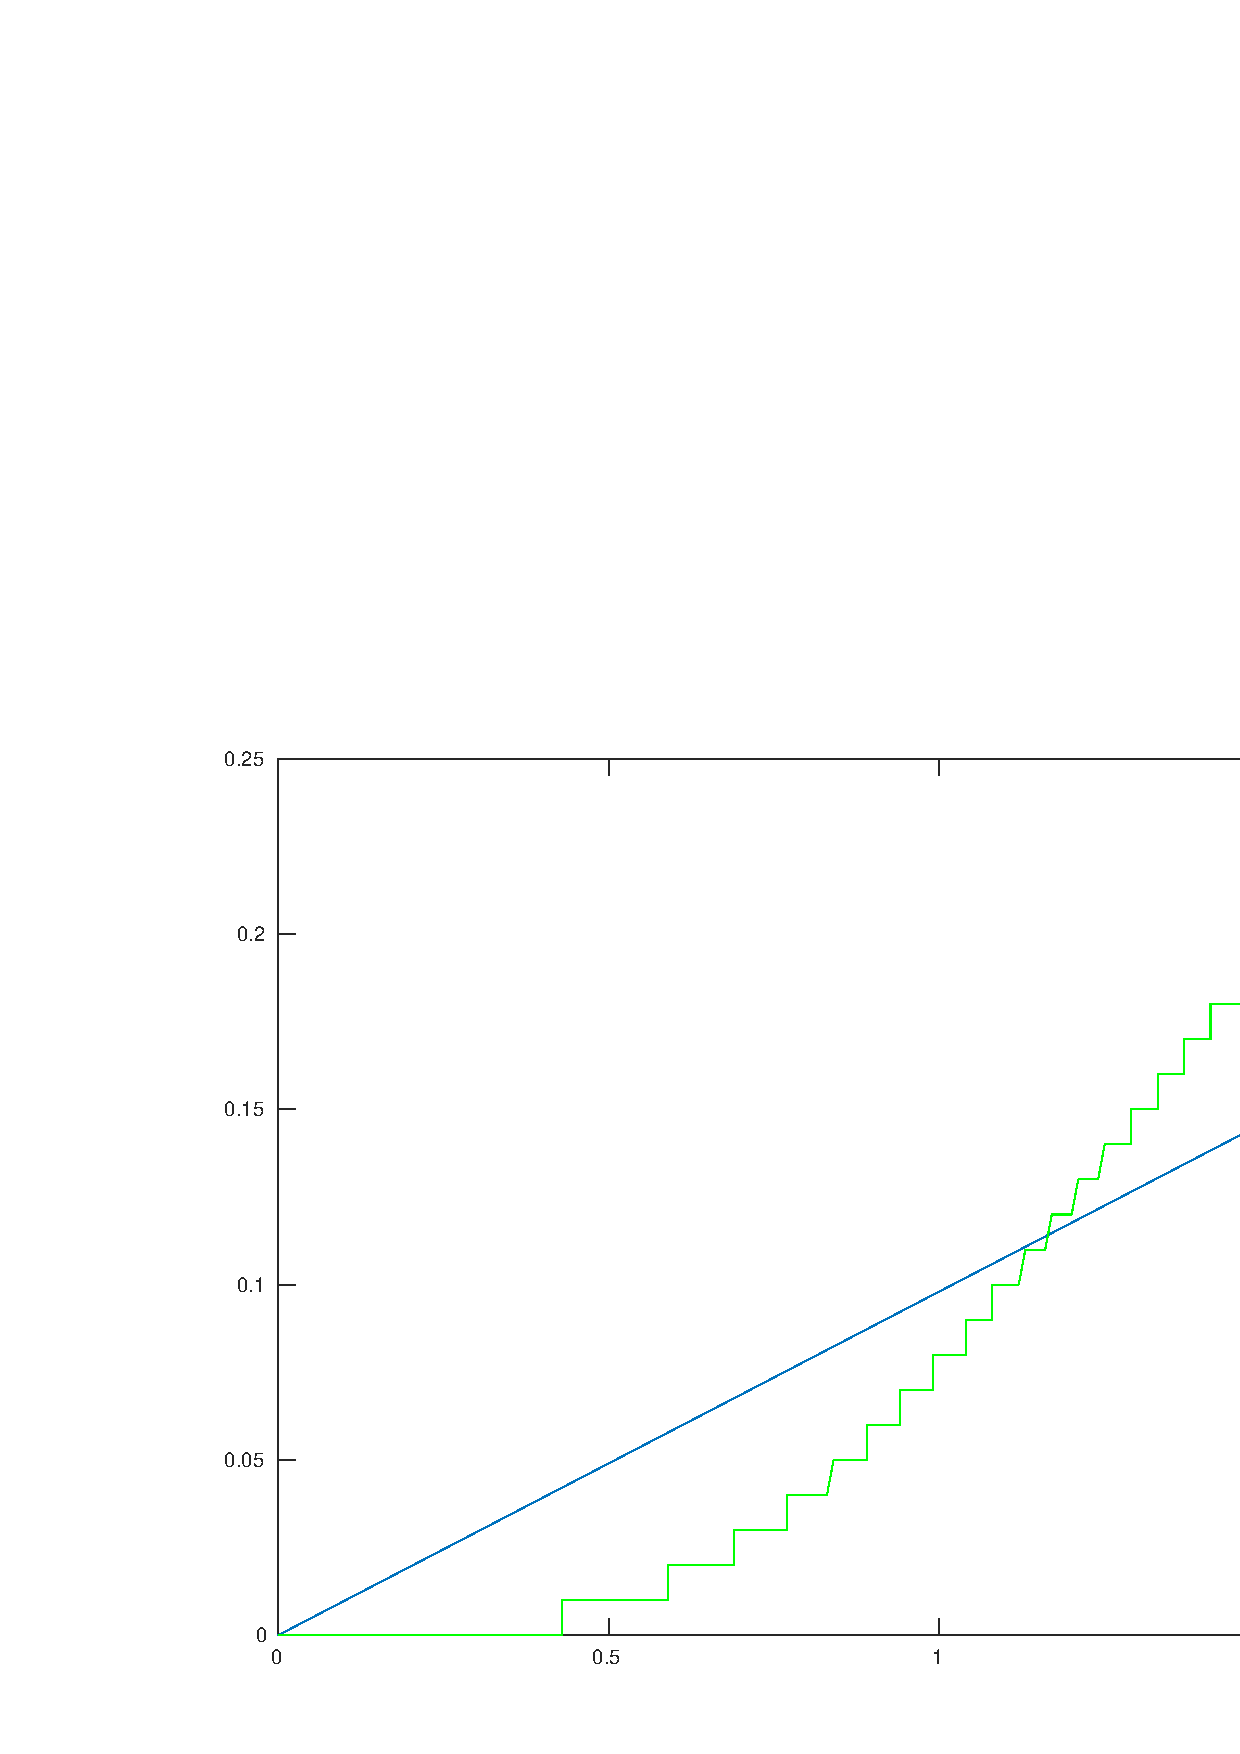
\includegraphics[width = 0.8\textwidth]{task17_spatial.png}
 \end{center}

Below we see $d_p$ for when the angle correcting part of the line following controller is in use.

\begin{center}
  \includegraphics[width = 0.8\textwidth]{task17_dp_both.png}
 \end{center}
\section*{Task 18}

The hybrid automaton is defined by the 8-tuple $H=(Q,X,Init,f,D,E,G,R)$, whereat Q is the set of states, X the continous state space, Init the initial states $\subseteq Q \times X$, f the vector fields $Q \times X \rightarrow x$, D the domain $Q \rightarrow 2^x$, E the set of edges $\subseteq Q \times Q$, G the guards $E \rightarrow 2^x$ and R the resets $E \times X \rightarrow 2^x$. In our case, we defined the automaton like the following:\\

\begin{equation}
Q=\{q_p,q_g,q_i\}	
\end{equation}

\begin{equation}
X=\mathbb{R}^3	
\end{equation} 

\begin{equation}
X=\mathbb{R}^3	
\end{equation}

\begin{equation}
f:
\begin{cases}
f(q_p,[x,y]^T) = 0 \\
f(q_p,\theta) = \frac{R}{L}*u_\Psi \\
f(q_g,[x,y]^T) = R*u_\omega*[\cos{\theta},\sin{\theta}]^T \\
f(q_g,\theta) = 0\\
f(q_i,[x,y]^T) = 0 \\
f(q_i,\theta) = 0\\
\end{cases}
\end{equation}

\begin{equation}
D:
\begin{cases}
D(q_p)=\{\theta\in[-\pi, \pi]: \theta\neq\theta^R, [x,y]^T\in\mathbb{R}^2\}\\
D(q_g)=\{\theta\in[-\pi, \pi]: \theta=\theta^R, [x,y]^T\in\mathbb{R}^2:[x,y]^T\neq[x_g,y_g]^T\}\\
D(q_i)=\{\theta\in[-\pi, \pi]: \theta=\theta^R,[x,y]^T\in\mathbb{R}^2:[x,y]^T=[x_g,y_g]^T\}\\
\end{cases}
\end{equation}
\begin{equation}
E=\{(q_p,q_g),(q_g,q_i),(q_i,q_p)\}
\end{equation}
\begin{equation}
G: 
\begin{cases}
G((q_p,q_g))=\{\theta\in[-\pi, \pi]: \theta=\theta^R\}\\
G((q_g,q_i))=\{[x,y]^T\in\mathbb{R}^2:[x,y]^T=[x_g,y_g]^T\}\\
G((q_i,q_p))=\{\theta\in[-\pi, \pi]: \theta\neq\theta^R\}\\
\end{cases}
\end{equation}

The initial state is the turning state $q_p$ as predefined in the assignment paper. The robot will rotate until it is pointing towards the goal with an error that is smaller than 2\degree. Once the system has switched from turning to line following state $q_g$ the robot will start driving towards the goal. The line following state is active until the robot is less than 5 cm away from the goal. A distance less than 5 cm to the goal is considered as having arrived the desired goal. Once the robot has arrived  at the goal it will switch to the idle state $q_i$, where it does remains standing still. In this way an oscillatory behaviour is prevented, where the robot would travel back and forth over the goal point. The robot will stand still at the goal until new goal coordinates are entered and the distance to the goal is larger than 5 cm again. This criteria is the guard condition to go to the initial state $q_p$ again, where the robot starts rotating until it is pointing into the direction of the new goal.
The behaviour of the Automaton allows only one direction of transition. It will only transit 'forward' but never back to a previous state.

\section*{Task 19}



\section*{Task 20} %This task is about copying code to the arduino file

This task intentionally left blank.

\section*{Task 21}

When driving manually, you send a fixed PWM to the motors for a short time per click. This is in contrary to to the case of automatic/autonomous driving where the robot slows down when approaching the target. In order to drive accurately you have to have a very slow feedback from your eyes to your control finger in order not to drive too far or turn too much. This is obviously hard without implementing a more sophisticated tele-op interface, such as proportional throttle.

\section*{Task 22}

As expected, the simulation results were far from identical to the results when trying it out practically. Two major issues limited our performance when applying the control strategy to the nexus robot. One was that we hadn't calibrated $p$ in equation \eqref{eq:vp} properly, causing it to not follow a path but just driving straight and thus being very vulnerable to bad starting angles. The second issue was our stopping conditions. In the simulation it worked well with the small tolerances we used, this didn't work as well in practice. First of all, we forced the robot to be within a certain distance from the goal both in $x$ and $y$ direction. In the simulation case the robot had reached its goal if it was at most 5 cm from the goal in $x$ and $y$. A smarter solution would be to pay attention to the angle to the goal. For instance, if the robot drives from $[x,y] = [0.0,0.0]$ to $[x,y] = [1.0,0.0]$, it should rather stop at $[x,y] = [1.0,0.1]$ than $[x,y] = [0.95,0.05]$, trying to modify its position. When stopping at $[x,y] = [1.0,0.1]$, since this case used straight corridors, it won't matter when driving to the next point which probably will be $\pi $ radians off. These are of course just example tolerances and attention has to be paid to the width of corridors and such so that the robot is still able to continue forward.

In the end, differences between simulation and real life usually involves that some events weren't modelled. Easy things like measurement noise, wheel size discrepancies and motor/wheel non-linearities from friction or battery voltage. But also stochastic events such as floor slip. In order to make your robot work well you always have to tune your controller on the real system and not spend too much time in simulation.



%%%%%%%%%%%%%%%%%%%%%%%%%%%%%%%%%%%%%%%%%%%%%%%%%%%%%%%%%%%%%%%%%%%%%%%%%%%%%%%%%%%
% The bibliography
%%%%%%%%%%%%%%%%%%%%%%%%%%%%%%%%%%%%%%%%%%%%%%%%%%%%%%%%%%%%%%%%%%%%%%%%%%%%%%%%%%%
%\bibliography{Bibliography_template} %Read the bibliography from a separate file

%\begin{thebibliography}{99}
%\bibitem[Khalil(2002)]{Khalil:2002:Nonlinear-systems:vh}
%Hassan~K Khalil.
%\newblock \emph{Nonlinear systems}.
%\newblock Prentice Hall, Upper Saddle river, 3. edition, 2002.
%\newblock ISBN 0-13-067389-7.
%
%\bibitem[Oetiker et~al.(2008)Oetiker, Partl, Hyna, and
%  Schlegl]{Oetiker:2008:TheNotSoShortIntroductiontoLaTeXe}
%Tobias Oetiker, Hubert Partl, Irene Hyna, and Elisabeth Schlegl.
%\newblock \emph{The Not So Short Introduction to \LaTeXe}.
%\newblock Oetiker, OETIKER+PARTNER AG, Aarweg 15, 4600 Olten, Switzerland,
%  2008.
%\newblock http://www.ctan.org/info/lshort/.
%
%\bibitem[Sastry(1999)]{Sastry:1999:Nonlinear-systems:-analysis-stability-and-c%
%ontrol:xr}
%Shankar Sastry.
%\newblock \emph{Nonlinear systems: analysis, stability, and control},
%  volume~10.
%\newblock Springer, New York, N.Y., 1999.
%\newblock ISBN 0-387-98513-1.
%\end{thebibliography}


\end{document}      % End of the document
